\documentclass{article}
\usepackage[utf8]{inputenc}
\usepackage{graphicx}
\usepackage{multicol}
\usepackage{caption}
\usepackage{makecell}
\usepackage{verbatim}
\usepackage[hidelinks]{hyperref}
\hypersetup{
    colorlinks=true,
    linkcolor=blue,     
    urlcolor=blue,
    }

\vspace{\stretch{1}}

\title{\LARGE Parallel Image Composition \\
\large Elaborato Parallel Programming For Machine Learning}
\author{Nicol\'o Pollini, Francesco Fantechi}
\date{A.A. 2022-2023}

\begin{document}

\maketitle

\begin{figure}[!h]
\centering

\includegraphics[width=4cm, height=4cm]{"Immagini/LogoUnifi.PNG"}
\end{figure}

\begin{center}
\textbf{\large UNIVERSITA' DEGLI STUDI DI FIRENZE \\
Facolta di Ingegneria \\
\normalsize Corso di Laurea Magistrale in Ingegneria Informatica}
\end{center}

\vspace{\stretch{1}}

\newpage

% Indice
\tableofcontents

\newpage

\section{Obiettivo}

L'obiettivo di questo progetto è quello di parallelizzare un algoritmo di Data Augmentation che effettua composizioni di immagini tramite il framework OpenMP e le librerie di Python che permettono il multiprocessing e confrontare i vari metodi valutando gli speedup ottenuti rispetto alle loro esecuzioni sequenziali.

\section{Data Augmentation}

La Data Augmentation \'e un insieme di processi atti ad aumentare gli elementi di un dataset senza raccogliere nuovi dati. Queste operazioni consistono infatti nell'effettuare cambiamenti controllati agli elementi del dataset ottenendo così copie modificate dei dati già essitenti. Questa tecnica trova un largo impiego nell'addestramento delle reti neurali quando i dati a disposizione non sono numericamente sufficienti e raccoglierne di nuovi risulterebbe troppo costoso o addirittura infattibile.\\
Nel nostro esperimento i dati da aumentare corrispondono a delle immagini raffiguranti dei quokka e per ottenerne di nuovi \'e stato effettuato un processo di Image Composition. Partendo da cinque immagini di background di dimensione $ 483\times594 $ pixel, sono state infatti generate nuove immagini andando ad applicare sopra di esse in punto randomico un'ulteriore immagine di dimensione $ 298\times350 $ pixel dopo avergli applicato una trasparenza anch'essa casuale. (vedi figura \ref{Images})  

\begin{figure}[!h]
\centering
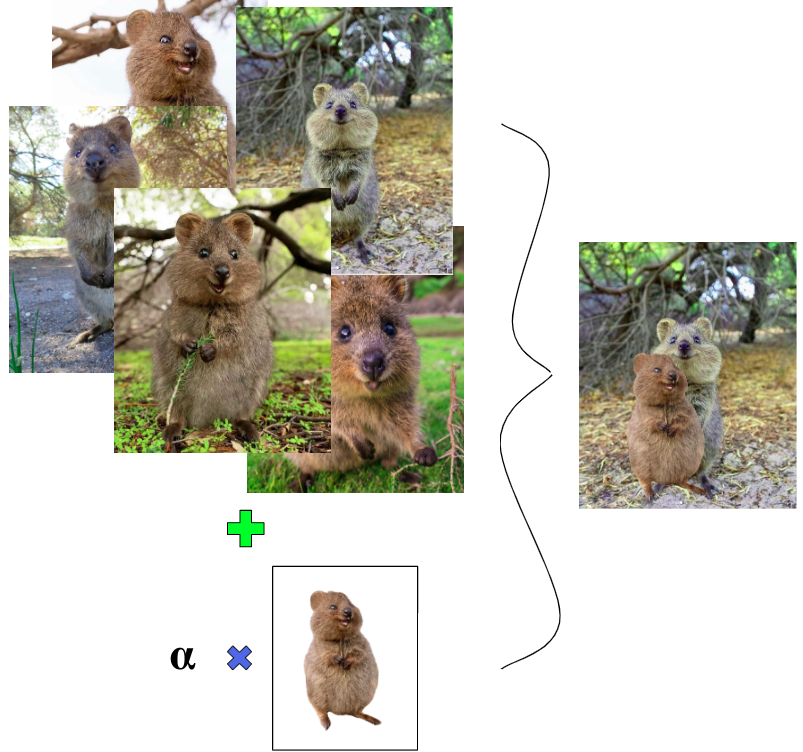
\includegraphics[width= 8.5cm]{"Immagini/Images.PNG"}
\caption{Data Augmentation mediante Image Composition}
\label{Images}
\end{figure}

\newpage

\section{Codice e implementazione}

Il progetto è stato implementato nei linguaggi C++ e Python ed \'e stato eseguito su due diverse macchine le cui caratteristiche sono riportate in Tabella \ref{Technical Specifications}. Il codice \'e stato versionato tramite la piattaforma GitHub ed \'e reperibile ai siti:\\
\url{https://github.com/francesco-ftk/Image_Composition_OpenMP.git} \\
\url{https://github.com/francesco-ftk/Image_Composition_Multiprocessing.git}\\
\\
\noindent Il progetto pu\'o essere suddiviso in tre parti:
\begin{enumerate}
\item Implemenatazione dell'agoritmo di Image Composition sequenziale
\item Parallelizzazione dell'algoritmo tramite il framework OpenMP in C++
\item Parallelizzazione dell'algoritmo tramite le librerie di multiprocessing in Python
\end{enumerate}

\subsection{Image Composition Sequenziale}

Date le immagini di partenza e un parametro \textit{“transformations”} indicativo del numero di nuove immagini volute, l'Image Composition \'e stata eseguita andando a scegliere ad ogni nuova trasformazione un'immagine fra quelle possibili di background in modo randomico. A queste \'e stata quindi aggiunta in posiszione randomica l'immagine di foreground con una trasparenza uniformemente scelta nell'intervallo $ [128,255] $. Le immagini sono state lette, editate e salvate tramite la libreria OpenCV. In figura \ref{Sequential} \'e riporato un estratto del codice sequenziale che implementa l'Image Composition scritto in linguaggio Python. Nonostante la sintassi diversa, la versione in scritta in linguaggio C++ si presenta praticamente uguale per quanto riguarda la forma.\\
I tempi di completamento in secondi per il codice scritto in linguaggio Python e in millisecondi per il codice scritto in C++ sono riportati in tabella \ref{Timings_Python} e \ref{Timings_C++}. 

\begin{figure}[!h]
\centering
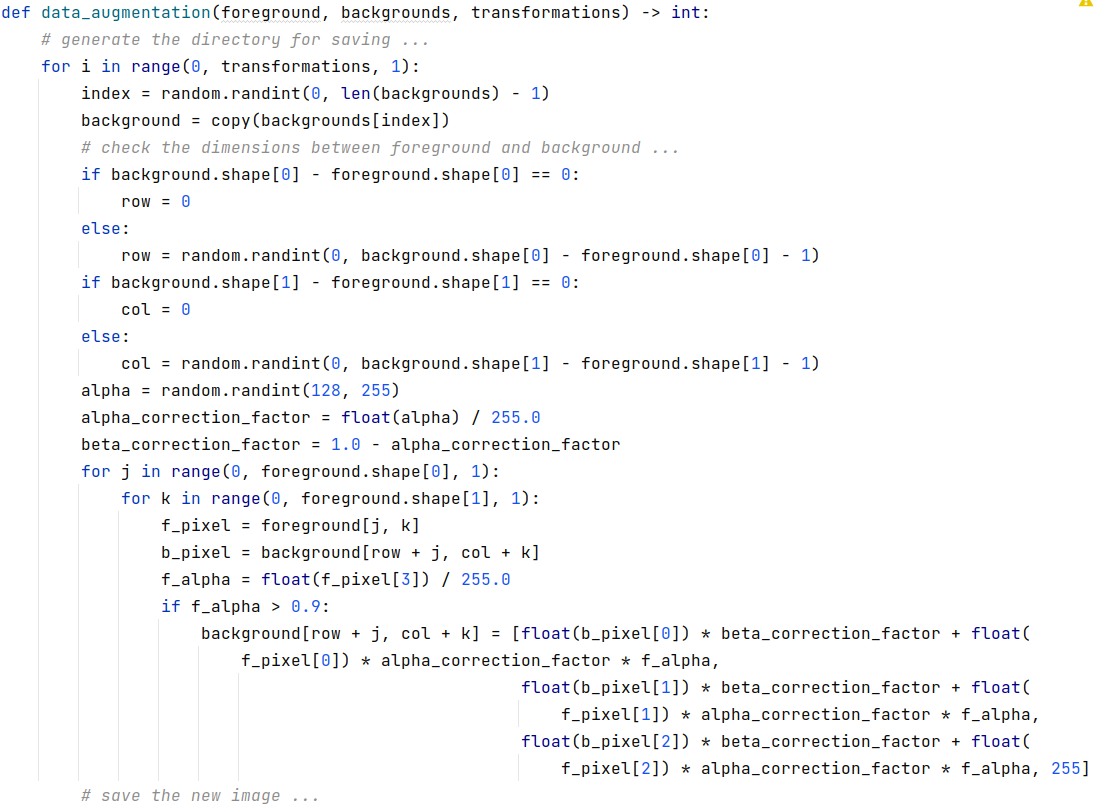
\includegraphics[width= 13cm]{"Immagini/Sequential.PNG"}
\caption{Codice Python che implementa l'algoritmo di Image Composition}
\label{Sequential}
\end{figure}

\newpage


\subsection{OpenMP}
OpenMP \'e un framework che permette di parallelizzare una porzione di codice in modalit\'a implicit threading attraverso delle direttive “pragma”.\\
Nel nostro esperimento la tipologia di parallelizzazione utilizzata \'e stata di tipo coarse-grained, ossia anzich\'e parallelizzare il processo stesso di composizione delle immagini, viene parallelizzato il ciclo esterno. In altre parole, ogni thread genera una porzione delle immagini di output richieste tramite il parametro \textit{“transformations”}, in modo che ogni nuova immagine venga ottenuta in modo indipendente dalle altre. L'algoritmo risuta quindi imbarazzantemente parallelo e quindi facilmente parallelizzabile in quanto i thread non necessitano di comunicare o scambiare informazioni fra di loro (Vedi figura \ref{OpenMP}).

\noindent Il numero di thread usati \'e stato calcolato aggiungendo un
$50\%$ al numero complessivo di Core posseduti dalla macchina utilizzata considerando l’Hyper-Threading (vedi Tabella \ref{Technical Specifications}). I tempi di esecuzione in millisecondi della Macchina $ 1 $ (vedi Tabella \ref{Technical Specifications}) presi in modialit\'a “Debug” sono riportati in Tabella \ref{Timings_C++}. Con questi tempi $t_{p}$ e quelli presi tramite l’implementazione sequenziale $t_{s}$ sono stati successivamente calcolati gli speedup tramite la formula $S=t_{s}/t_{p}$. Questi ultimi sono osservabili in Tabella \ref{Speedups}.
\newpage
\noindent In Figura \ref{Timings_Varying_Threads} \'e riportato un grafico che mostra i tempi di esecuzione in millisecondi per la Macchina $ 1 $ (vedi Tabella \ref{Technical Specifications}) al variare del numero dei thread per genereare $ 1800 $ immagini.\\ In Figura \ref{Speedups_Varying_Transformations} \'e possibile osservare invece un grafico che mostra gli speedups ottenuti dalla Macchina $ 1 $ (vedi Tabella \ref{Technical Specifications}) al variare del numero di immagini generate utilizzando $ 18 $ thread.

\begin{figure}[!h]
\centering
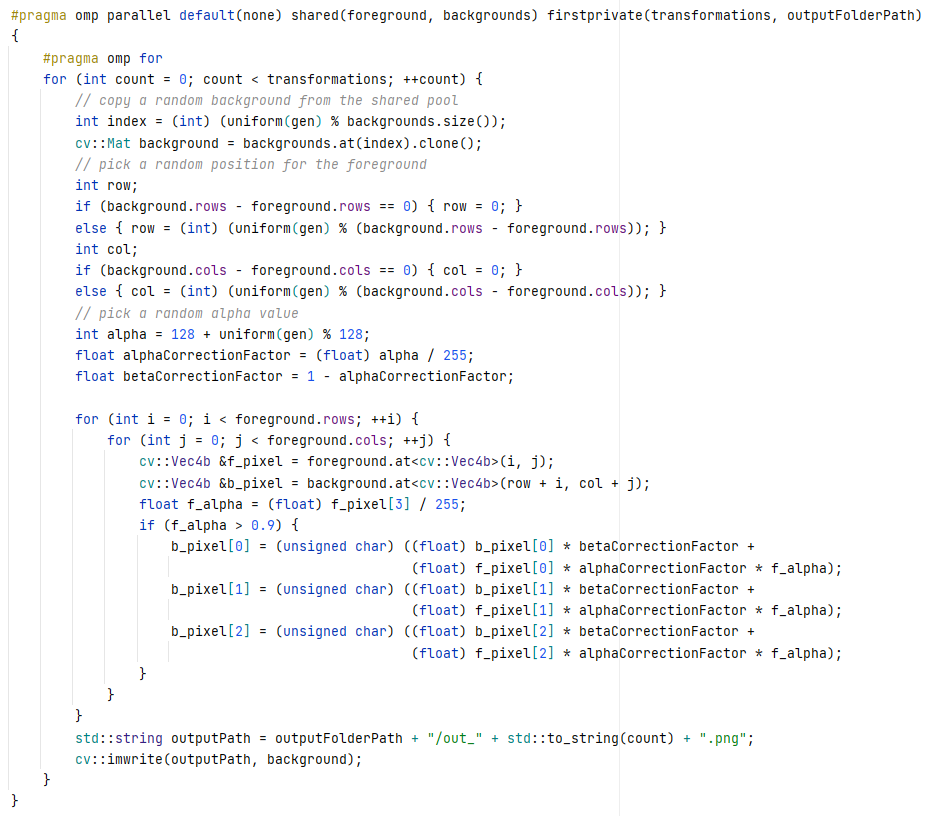
\includegraphics[width= 13cm]{"Immagini/OpenMP.PNG"}
\caption{Parallelizzazione tramite framework OpenMP in C++}
\label{OpenMP}
\end{figure}

\subsection{Multiprocessing}
A causa dell'interprete GIL (Global Interpretr Lock) che gestisce il garbage collector con dei contatori di riferimento sugli oggetti per determinare quando non sono pi\'u in uso, in Python non \'e possibile eseguire pi\'u di un thread contemporaneamente. Un modo per superare queste limitazioni di concorrenza pu\'o essere quello di istanziare dei sottoprocessi al posto dei thread. Ogni processo posseder\'a infatti il proprio GIL e potr\'a essere eseguito in modo asincrono su un core diverso ottenendo cos\'i il parallelismo. Il superamento delle restrinzioni di concorrenza va per\'o a discapito della performance in quanto istanziare i processi risulta molto pi\'u costoso ripetto a far partire dei thread.\\
Nel nostro esperimento sono stati implementati due metodi differenti per istanziare i sottoprocessi: il primo basato sulla libreria standard di Python Multiprocessing e il secondo tramite la libreria Joblib.\\
La libreria Multiprocessing permette di istanziare e far partire manualmente i processi su una certa funzione target passata alla loro creazione. Il lavoro \'e stato equamente suddiviso fra i vari processi. Ognuno di essi infatti riceve come argomenti le immagini di background e foreground e il parametro \textit{“transformations\_for\_process”} ottenuto dividendo il numero di trasformazioni volute per il numero di processi istanziati. Due implementazioni equivalenti del suo utilizzo sono riportate in figura \ref{Pool} e \ref{Multiprocessing}.
\\ In Figura \ref{Speedups_Varying_Transformations_Multiprocessing} \'e possibile osservare un grafico che mostra gli speedups ottenuti dalla Macchina $ 2 $ (vedi Tabella \ref{Technical Specifications}) al variare del numero di immagini generate utilizzando $ 12 $ processi.

\vspace{20px}

\begin{figure}[!h]
\centering
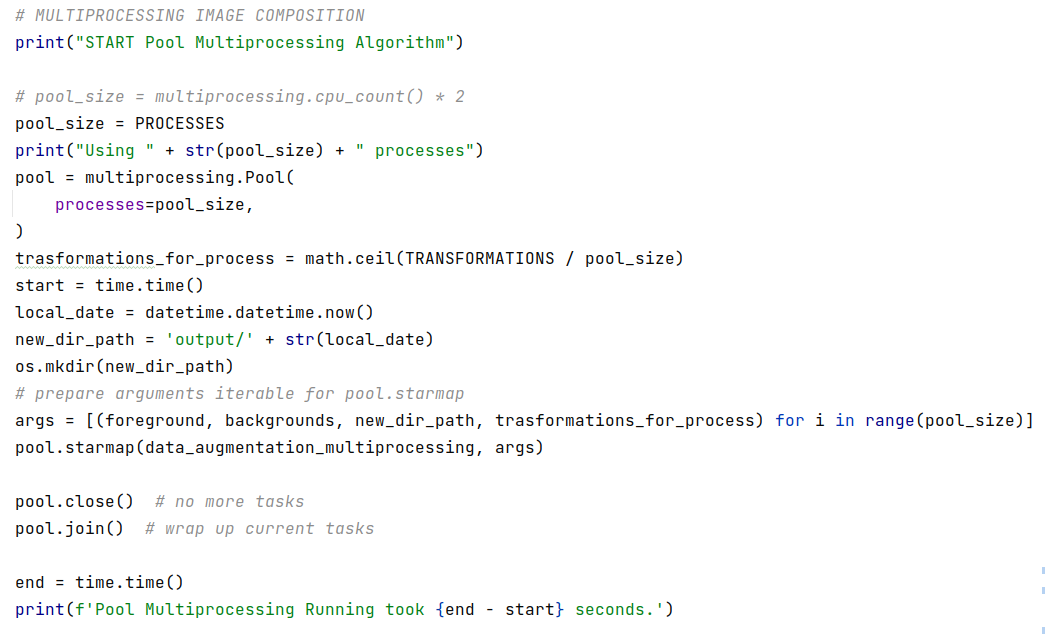
\includegraphics[width= 12.5cm]{"Immagini/Pool.PNG"}
\caption{Codice Python che utilizza la librearia Multiprocessing con Pooling}
\label{Pool}
\end{figure}

\begin{figure}[!h]
\centering
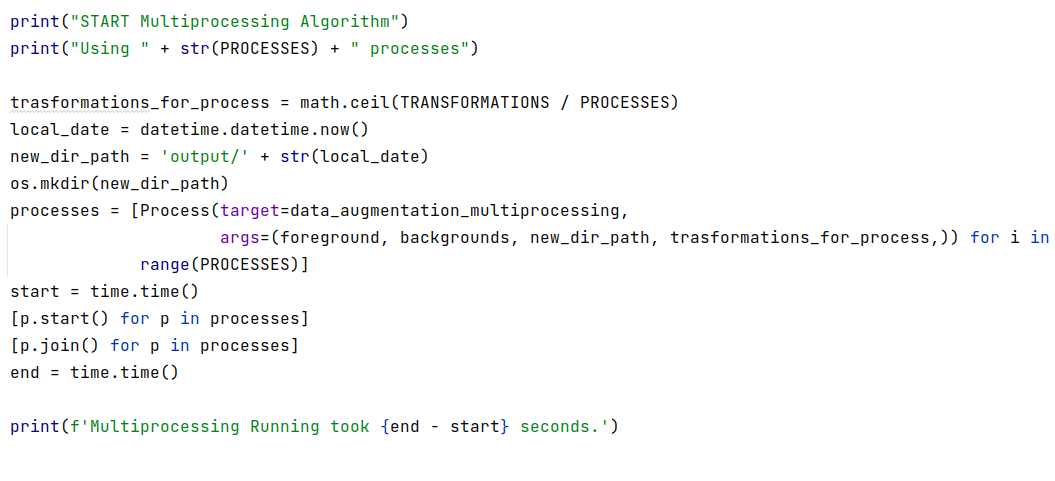
\includegraphics[width= 12.5cm]{"Immagini/Multiprocessing.PNG"}
\caption{Codice Python che utilizza la libreria Multiprocessing}
\label{Multiprocessing}
\end{figure}

\newpage

\noindent La libreria Joblib permette di parallelizzare mediante il multiprocessing programmi imbarazzantemente paralleli. I processi vengono eseguiti in modo asincrono sulla propria funzione target suddividendosi il lavoro in modo autonomo. Dato che ad ogni nuova esecuzione di un processo gli argomenti posseduti devono essere ripassati in ingresso alla funzione, per ridurre i costi ogni processo genera una nuova immagine alla volta e riceve gi\'a negli argomenti l'immagine di background da utilizzare e non l'intero dataset da cui scegliere. Il codice che implementa questa libreria \'e riportato in figura \ref{Joblib}.

\begin{figure}[!h]
\centering
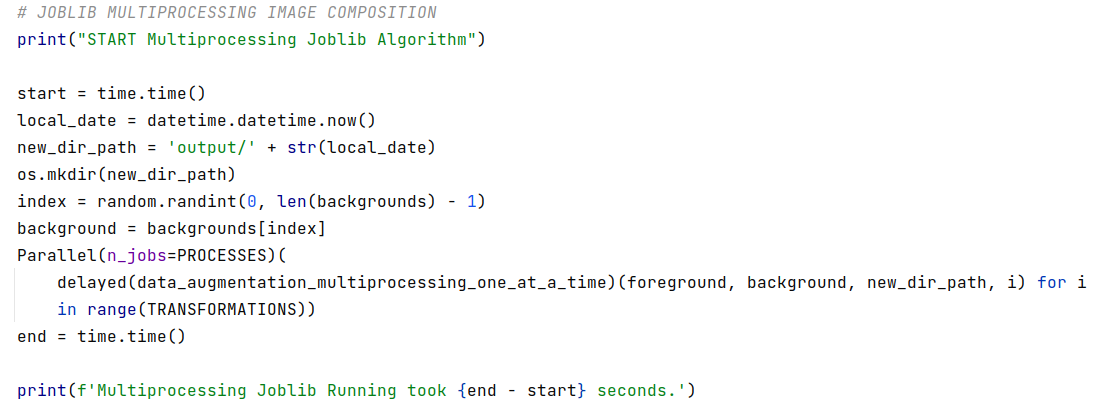
\includegraphics[width= 12.5cm]{"Immagini/Joblib.PNG"}
\caption{Codice Python che utilizza la libreria Joblib}
\label{Joblib}
\end{figure}

\noindent Il numero di processi istanziati \'e stato calcolato aggiungendo un $50\%$ al numero complessivo di Core posseduti dalla macchina utilizzata considerando l’Hyper-Threading (vedi Tabella \ref{Technical Specifications}). I tempi di completamento in secondi della Macchina $ 2 $ (vedi Tabella \ref{Technical Specifications}) sono riportati in Tabella \ref{Timings_Python}. Con questi tempi sono stati successivamente calcolati gli speedup di entrambi i metodi rispetto all'esecuzione sequenziale. Questi ultimi sono osservabili in Tabella \ref{Speedups}.

\newpage   

\section{Risultati}

\begin{center}
\captionof{table}{Machine's technical specifications} \label{Technical Specifications}
\begin{tabular}{|c|c|c|c|}
\hline
\multicolumn{4}{|c|}{Machine 1}\\
\hline
\thead{OS} & \thead{CPU} & \thead{Number of Core \\ with Hyper-Threading} & \thead{RAM}\\
\hline
\thead{Windows $ 10 $} & \thead{Intel(R) Core(TM) \\ i7-8750H} & \thead{$ 12 $} & \thead{$ 16 $ GB}\\
\hline
\multicolumn{4}{|c|}{}\\
\hline
\multicolumn{4}{|c|}{Machine 2}\\
\hline
\thead{OS} & \thead{CPU} & \thead{Number of Core \\ with Hyper-Threading} & \thead{RAM}\\
\hline
\thead{Ubuntu $ 20.04.5 $} & \thead{Intel(R) Core(TM) \\ i7-1165G7} & \thead{$ 8 $} & \thead{$ 16 $ GB}\\
\hline
\end{tabular}

\captionof{table}{Python Timings} \label{Timings_Python}
\begin{tabular}{|c|c|c|c|c|}
\hline
\multicolumn{5}{|c|}{Machine 2}\\
\hline
\thead{Number of Images} & \thead{Sequential} & \thead{Joblib} & \thead{Pool Multiprocessing} & \thead{Multiprocessing} \\
\hline
\thead{$ 1200 $} & \thead{$ 122.1s $} & \thead{$ 143.9s $} & \thead{$ 52.1s $}  & \thead{$ 50.7s $}\\
\hline
\end{tabular}

\captionof{table}{C++ Timings} \label{Timings_C++}
\begin{tabular}{|c|c|c|}
\hline
\multicolumn{3}{|c|}{Machine 1}\\
\hline
\thead{Number of Images} & \thead{Sequential} & \thead{OpenMP} \\
\hline
\thead{$ 1800 $} & \thead{$ 88974ms $} & \thead{$ 14832ms $}\\
\hline
\end{tabular}

\captionof{table}{Speedups} \label{Speedups}
\begin{tabular}{|c|c|c|c|}
\hline
\multicolumn{4}{|c|}{Machine 1}\\
\hline
\multicolumn{4}{|c|}{OpenMP}\\
\hline
\multicolumn{4}{|c|}{$ 6.0 $}\\
\hline
\multicolumn{4}{|c|}{}\\
\hline
\multicolumn{4}{|c|}{Machine 2}\\
\hline
\multicolumn{1}{|c|}{\hspace*{0.5cm}Joblib\hspace*{0.5cm}} & \multicolumn{2}{c|}{Pool Multiprocessing} & \multicolumn{1}{c|}{Multiprocessing}\\
\hline
\multicolumn{1}{|c|}{$ 0.9 $} & \multicolumn{2}{c|}{$ 2.3 $} & \multicolumn{1}{c|}{$ 2.4 $}\\
\hline
\end{tabular}

\newpage

\begin{figure}[!h]
\centering
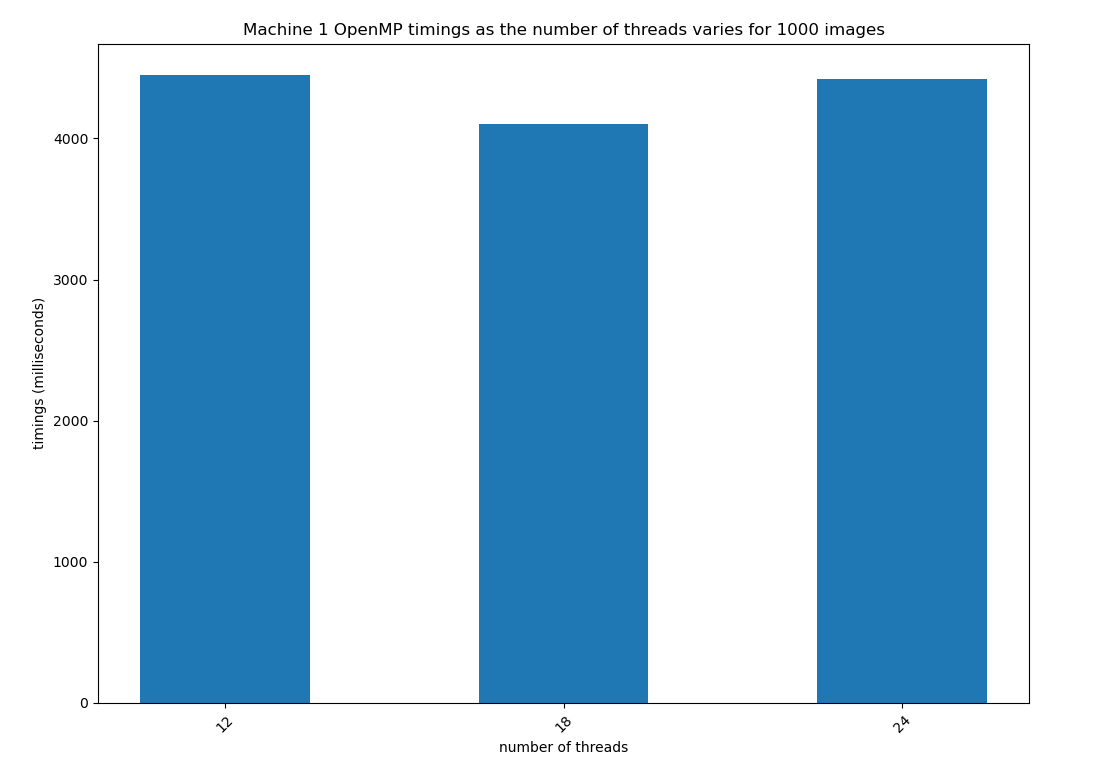
\includegraphics[width= 12cm]{"Immagini/Timings_Varying_Threads.PNG"}
\caption{Machine $ 1 $ OpenMP timings as the number of threads varies}
\label{Timings_Varying_Threads}
\end{figure}

\begin{figure}[!h]
\centering
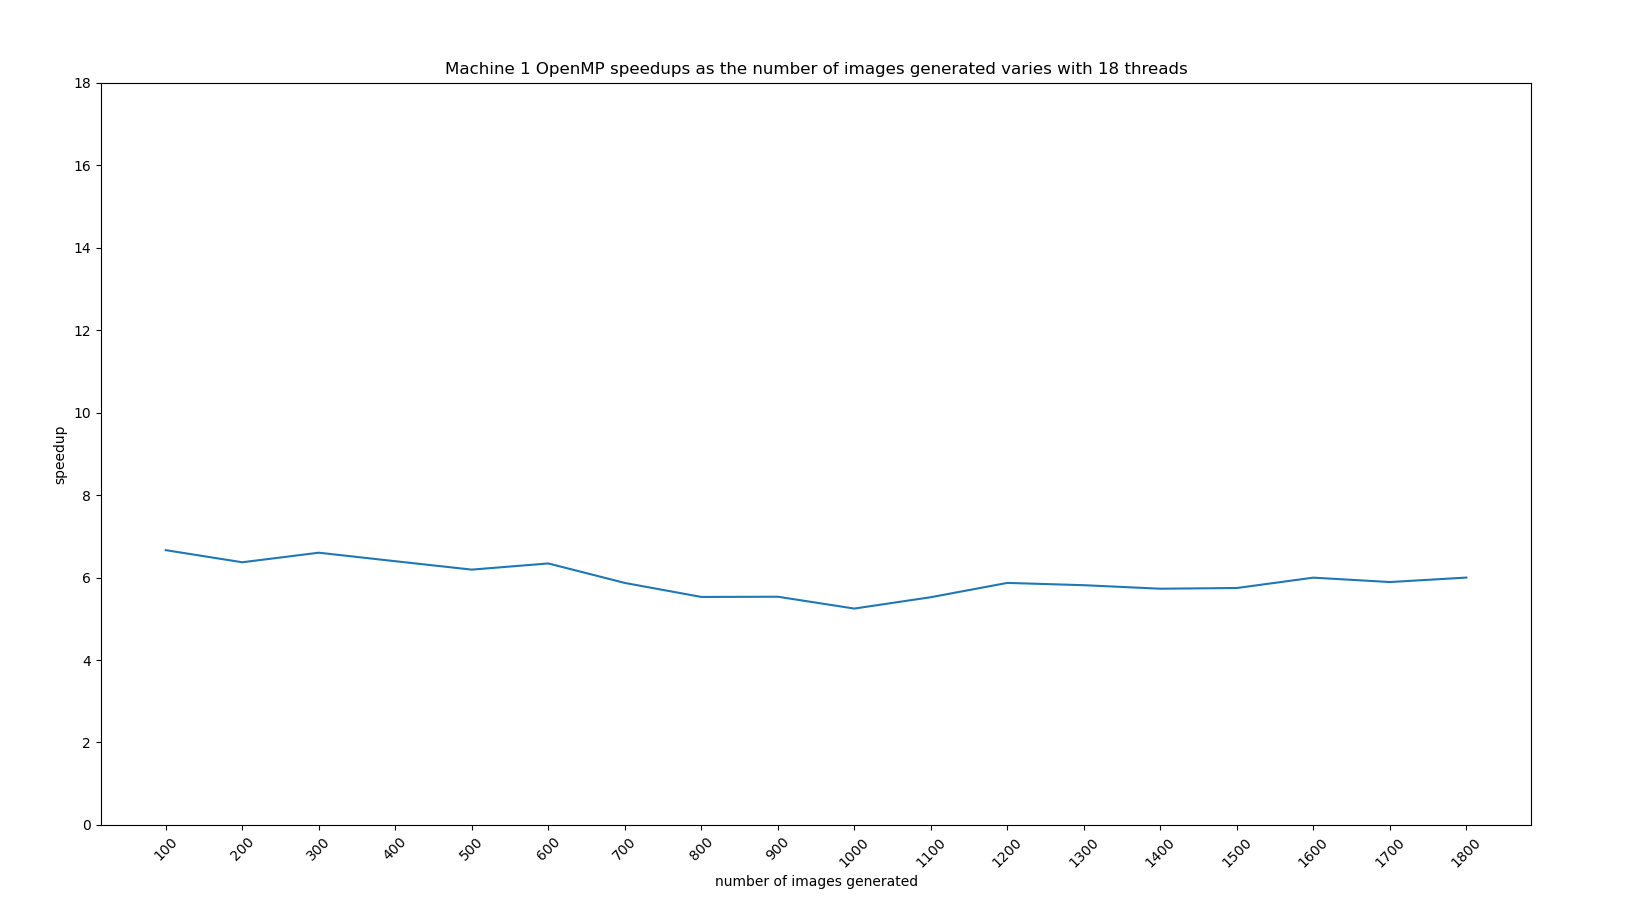
\includegraphics[width= 13cm]{"Immagini/Speedup_Varying_Transformations.PNG"}
\caption{Machine $ 1 $ OpenMP speedups as the number of generated images varies}
\label{Speedups_Varying_Transformations}
\end{figure}

\end{center}

\newpage

\begin{center}

\begin{figure}[!h]
\centering
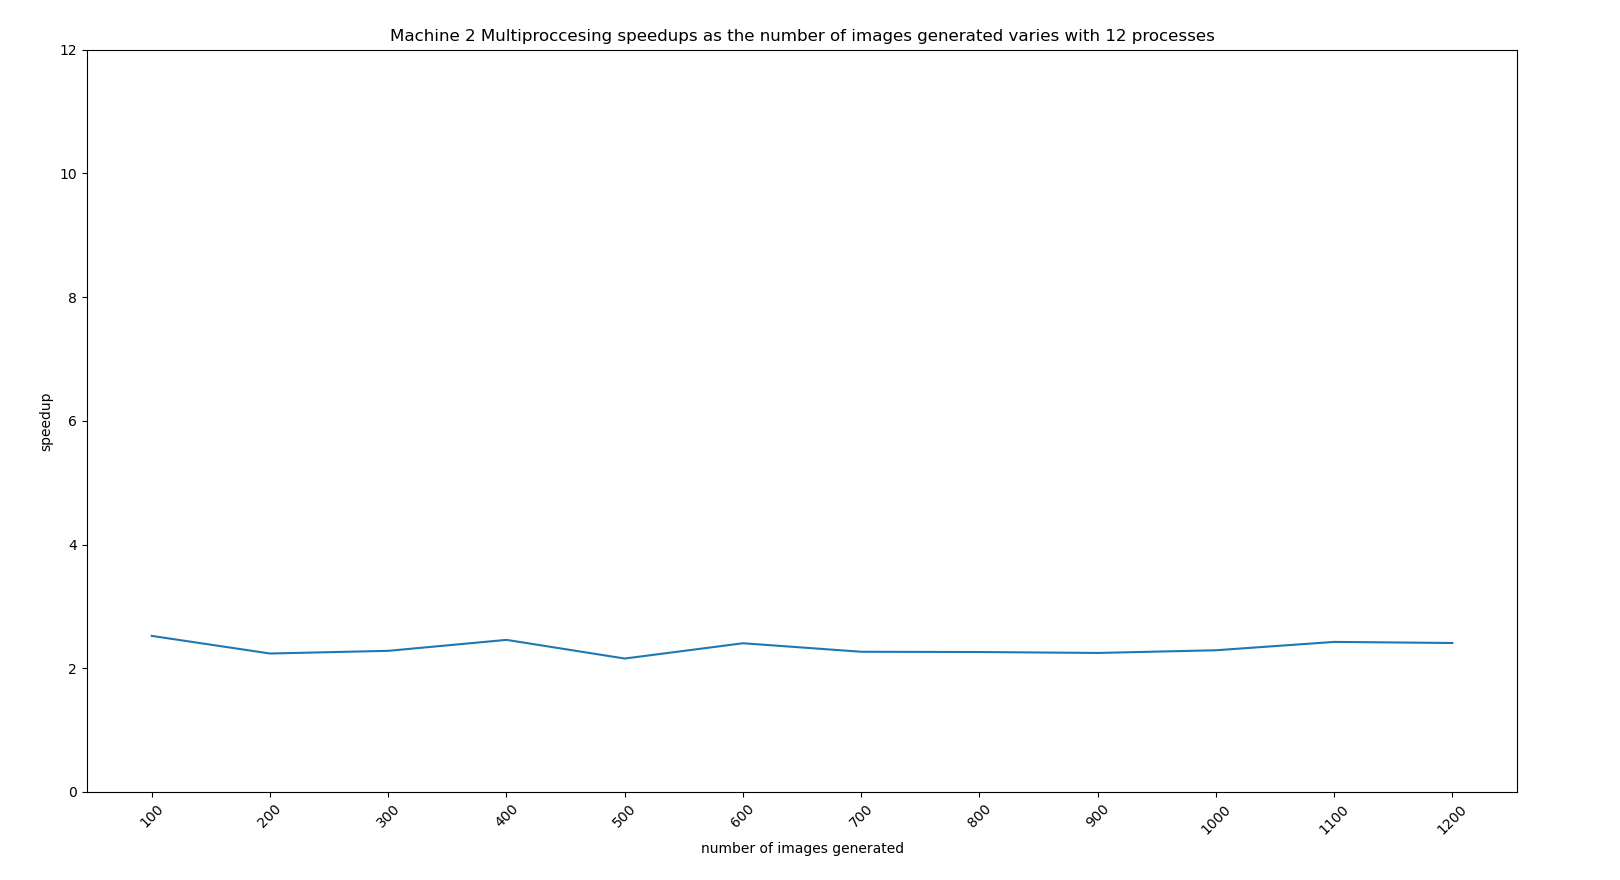
\includegraphics[width= 13cm]{"Immagini/Speedup_Varying_Transformations_Multiprocessing.PNG"}
\caption{Machine $ 2 $ Multiprocessing speedups as the number of generated images varies}
\label{Speedups_Varying_Transformations_Multiprocessing}
\end{figure}

\end{center}


\section{Analisi e Conclusioni}

Come previsto, la parallelizzazione ha permesso di ottenere uno speedup sublineare, che nel caso di OpenMP \'e molto vicino al numero di core fisici presenti nella macchina utilizzata. Questo risultato può essere motivato grazie ad una parallelizzazione effettuata dividendo il carico di lavoro in modo equo sui thread disponibili. Se il numero di immagini da generare fosse stato troppo basso sarebbe stato possibile osservare una diminuzione delle performance di parallelizzazione a causa di uno sbilanciamento del carico di lavoro sui thread; tuttavia, come \'e possibile apprezzare dal grafico \ref{Speedups_Varying_Transformations}, se il numero di trasformazioni rimane abbastanza alto, lo speedup rimane invece stabile al variare del carico di lavoro.\\
Lo stesso comportamento \'e apprezzabile in figura \ref{Speedups_Varying_Transformations_Multiprocessing} per la parallelizzazione in Python tramite la la libreria di Multiprocessing. In questo caso per\'o, essendo i processi più costosi da far partire rispetto ai thread e possedendo la Macchina $ 2 $ (vedi Tabella \ref{Technical Specifications}) un numero inferiore di core, lo speedup risulta nettamente inferiore a quello ottenuto con OpenMP.\\
Come \'e possibile osservare in Tabella \ref{Speedups}, lo speedup risulta inesistente invece utilizzando la libreira Joblib forse per il costo maggiore dei processi e il modo di instanziarli nuovamente di quest'ultima ad ogni nuovo task.

\end{document}